\section{Curva de descarga}
\label{app:curva-descarga}

La figura~\ref{fig:discharge-curve} muestra la curva de descarga de las baterías del \MEE cuando el \emph{Tiempo de espera entre mensajes} (ver Sección~\ref{sec:params-exterior}, \textit{\nameref{sec:params-exterior}}) se ha establecido en 1 minuto.
Con dicha frecuencia de mensajes, y con baterías en perfectas condiciones, el \ME tarda aproximadamente 18 días en alcanzar el umbral de batería bajo por defecto (4,72 V), y menos de 21 días en descargarse por completo. 

Dado el reducido consumo de batería del \MEE cuando se encuentra en reposo, es posible alargar la duración de las baterías de forma notable incrementando el \emph{Tiempo de espera entre mensajes} a varios minutos. Por ejemplo, con un \emph{Tiempo de espera entre mensajes} de 5 minutos ---el valor por defecto--- la batería debería durar entre 10 y 12 semanas.

\begin{figure}[H]
  \centering
  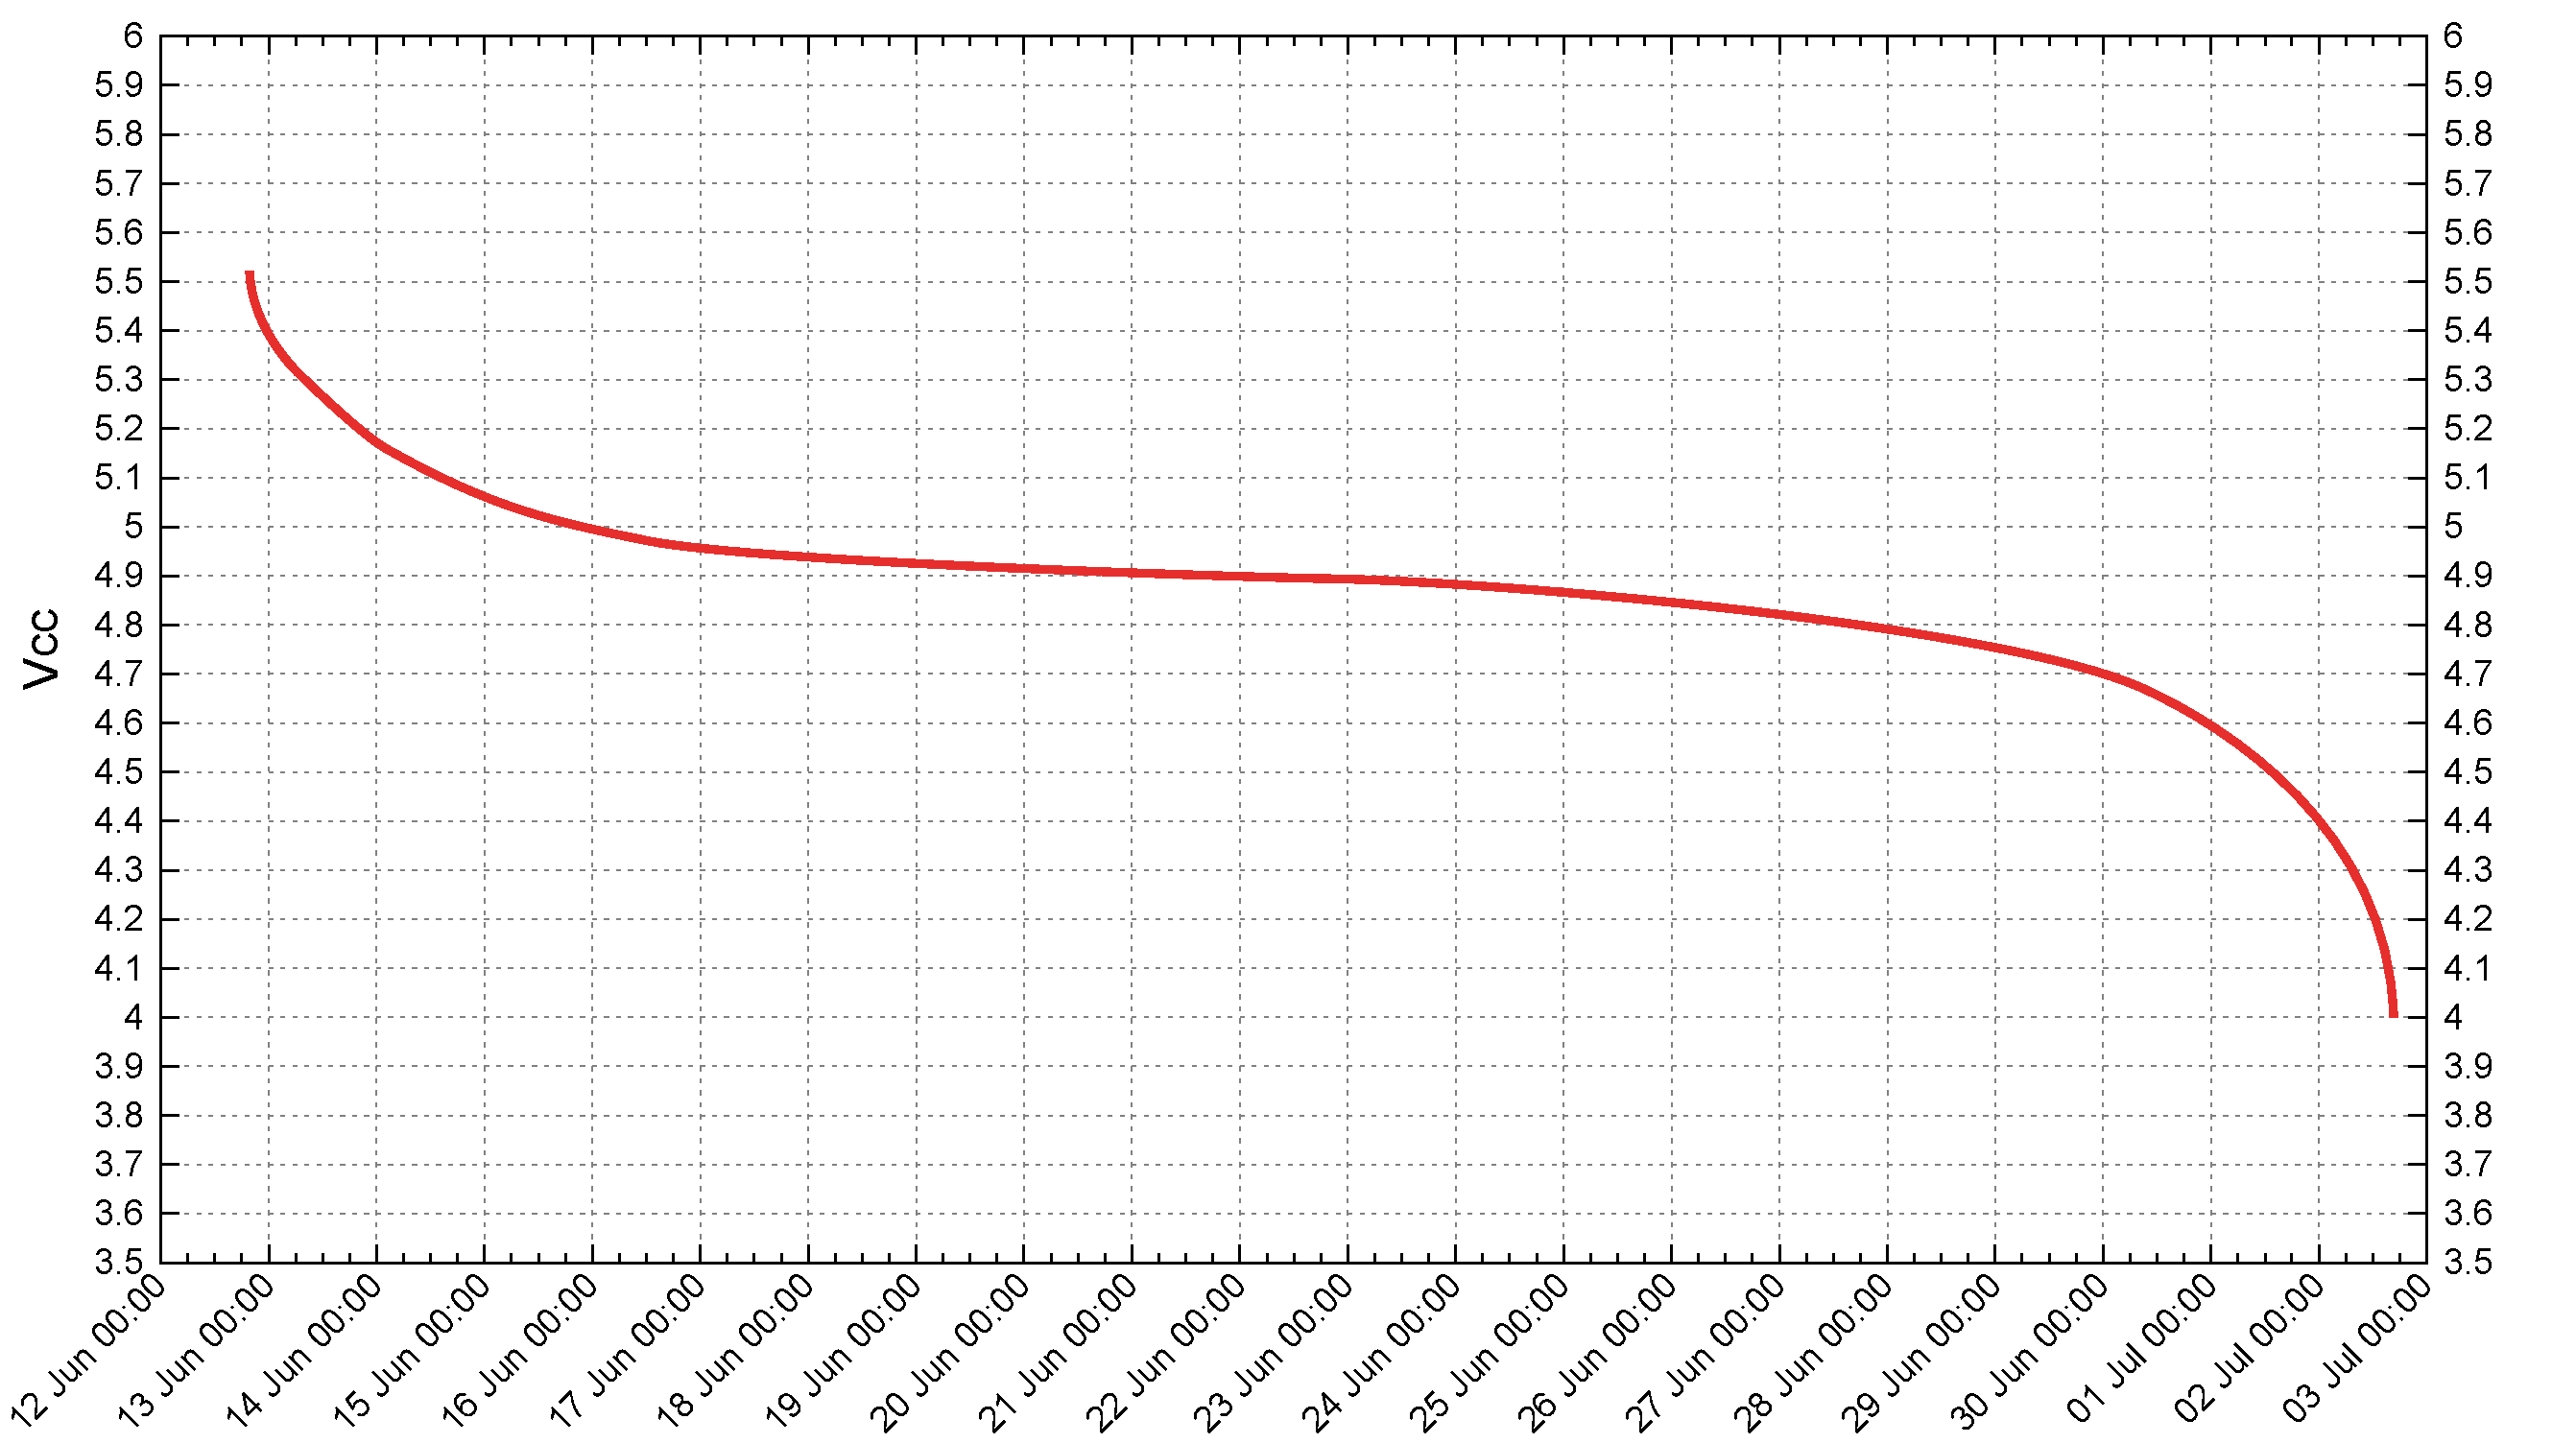
\includegraphics[width=1\columnwidth]{images/discharge-curve}
  \caption{Curva de descarga}
  \label{fig:discharge-curve}
\end{figure}

